% !TEX root = ../../ozan_sener_thesis.tex

\begin{figure}[t]
\centering
\subfigure[original graph]{\label{a}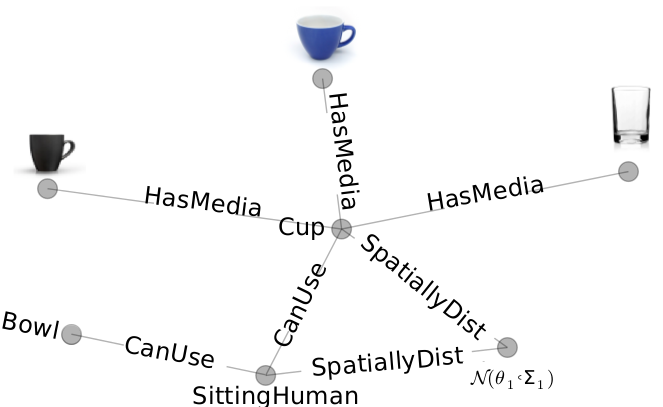
\includegraphics[width=0.48\textwidth]{before.png}}~\subfigure[feed insertion]{\label{a}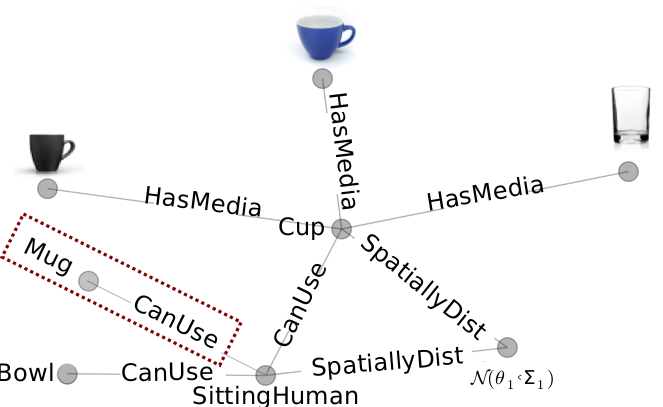
\includegraphics[width=0.48\textwidth]{insert.png}}

\subfigure[after $merge(Mug,Mug^\prime) \rightarrow Mug \circ split(Cup)\rightarrow(Cup,Mug^\prime)$]{\label{a}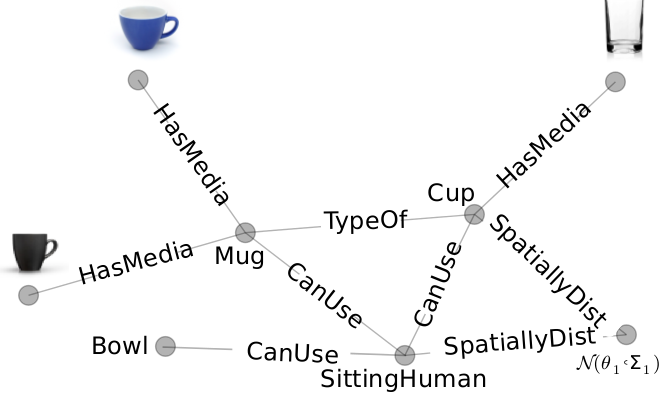
\includegraphics[width=0.48\textwidth]{after.png}}
\caption{\textbf{Visualization of inserting new information.} We insert `\emph{Sitting human can use a mug}' and \robobrain{} infers the necessary split and merge operations on the graph. In (a) we show the original sub-graph, In (b) information about a \emph{Mug} is seen for the first time and the corresponding node and edge are inserted, In (c) inference algorithm infers that previously connected cup node and  cup images are not valid any more, and it splits the $Cup$ node into two nodes as $Cup$ and $Mug^\prime$ and then merges $Mug^\prime$ and $Mug$ nodes.}
\label{insertgraph}
\end{figure}


\section{Knowledge Engine: Formal Definition}
\label{sec:graph}

In this section we present the formal definition of \mbox{\robobrain{}}.
\robobrain{} represents knowledge as a directed graph $\mathcal{G}=(V,E)$.
The vertices $V$ of the graph stores concepts that can  be of a variety
of types such as images, text, videos, haptic data, or  learned entities such as affordances, deep learning features, parameters, etc.
The edges $E \subseteq V\times V\times C$ are directed and represents the relations between concepts. Each edge has an edge-type from a set $C$ of possible edge-types.

An edge $(v_1,v_2,\ell)$ is an ordered set of two nodes $v_1$ and $v_2$ and an edge-type  $\ell$.
%connected by an edge type $\ell$ from $v_1$ to $v_2$.
% in which it represent there exist an edge from node $v_1$ to node $v_2$ with type $l$.
Few examples of such edges are: $($StandingHuman, Shoe, \emph{CanUse}$)$,
$($StandingHuman, $\mathcal{N}(\mu,\Sigma)$, \emph{SpatiallyDistributedAs}$)$
and $($Grasping, DeepFeature$23$, \emph{UsesFeature}$)$. %These edges can be considered as (\emph{subject}, \emph{object}, \emph{predicate}) triplets.
We do not impose any constraints on the type of data that nodes can represent. However, we require the edges to be consistent with \robobrain{} edge set $C$. We further associate each node and edge in the graph with \textit{a feature vector representation} and a \textit{belief}. The feature vector representation of nodes and edges depend on their local connections in the graph, and their belief is a scalar probability over the accuracy of the information that the node or an edge represents. Tables~\ref{tbl:vertices} and~\ref{tbl:edges} show few examples of nodes and edge-types. A snapshot of the graph is shown in  Figure~\ref{fig:graph}.

\subsection{Creating the Graph}
Graph creation consists of never ending cycle of two stages namely, knowledge acquisition and inference. Within the knowledge acquisition stage, we collect data from various sources and during the inference stage we apply statistical techniques to update the graph structure based on the aggregated data. We explain these two stages below.



\smallskip
\noindent{\textbf{Knowledge acquisition:}} \robobrain{} accepts new information in the form of set of edges, which we call a \textit{feed}. A \textit{feed} can either be from an automated algorithm crawling the Internet sources or from one of \robobrain{}'s partner projects.
We add a new \textit{feed} to the existing graph through a sequence of union operations performed on the  graph. These union operations are then followed by an inference algorithm.
More specifically, given a new \emph{feed} consisting of a set of $N$ edges \{$(v^1_1,v^1_2,\ell^1) \ldots (v^N_1,v^N_2,\ell^N)$\}, and the existing graph $G = (V,E)$. The graph union operations give a graph $G^\prime=(V^\prime,E^\prime)$ as follows:
\begin{equation}
\label{eq:update}
\begin{aligned}
V^\prime &= v^1_1 \cup v^1_2 \cup \ldots \cup v^N_1 \cup v^N_2 \cup V \\
E^\prime &=  (v^1_1,v^1_2,\ell^1) \cup \ldots \cup (v^N_1,v^N_2,\ell^N) \cup E
\end{aligned}
\end{equation}

%\noindent
%After the knowledge is acquired, we update the graph in the next step.

\smallskip
\noindent{\textbf{Inference on the Graph:}}
After adding the \textit{feed} to the graph using equation~\eqref{eq:update}, we perform inference to update the graph based on this new knowledge. The inference outputs a sequence of graph operations which are then performed on the graph. These graph operations modify the graph by adding new nodes or edges to the graph, deleting nodes or edges from the graph, merging or splitting nodes, etc.

We mention two graph operations here: \emph{split} and \emph{merge}. The split operation is defined as splitting a node into a set of two nodes. The edges having end points in the split node are connected to one of the resultant nodes using the inference algorithm. A merge operation is defined as merging two nodes into a single node, while updating the edges connected to the merged nodes. An example of such an update is shown in Figure \ref{insertgraph}. When a new information \emph{``sitting human can use a mug"} is added to the graph, it causes the \textit{split} of the \emph{Cup} node into two nodes: a \emph{Cup} and a \emph{Mug} node. These two are then connected by an edge-type \textit{TypeOf}. The graph update can be expressed through the following equation:
$$G^\star = split_{v_{s_1}} \circ merge_{v_{m_1},v_{m_2}} \circ \ldots \circ split_{v_{s_M}} \circ G^\prime$$

In the above equation $G^\star$ is the graph obtained after the inference. The goal of the inference steps is to modify the graph $G^\prime$ in a way that best explains the physical world. However, the graph that captures the real physical world is a  \textit{latent graph}, i.e., it is not directly observable.
For  example, the latent information that \emph{``coffee is typically in a container"} is partially observed through
many edges between the \emph{coffee} node and the nodes with \emph{container} images. Our graph construction can also be explained in a generative setting of having a latent graph with all the knowledge about physical word, and we only observe  noisy measurements in form of \textit{feeds}. In this chapter, we abstract the algorithmic details of inference and focus on the overall ideas involved in \robobrain{}, its architecture, and its application to robotics.
%system architecture and presenting the overall ideas in the RKE, and defer the details of inference algorithms and the latent graph to a later journal version.



\begin{table}
\caption{Some examples of different node types in our \robobrain{} graph. For full-list,
please see the code documentation.}
\label{tbl:vertices}
\begin{tabular}{ll}
Word & an English word represented as an ASCII string\\
DeepFeature & feature function trained with a Deep Neural Network\\
Image & 2D RGB Image\\
PointCloud & 3D point cloud\\
Heatmap & heatmap parameter vector\\
\end{tabular}
\end{table}
\begin{table}
\caption{Some examples of different edge types in our \robobrain{} graph. For full-list,
please see the code documentation.}
\label{tbl:edges}
\begin{tabular}{ll}
IsTypeOf & human \emph{IsTypeOf} a mammal \\
HasAppearance & floor \emph{HasAppearance} as follows (this image) \\
CanPerformAction & human \emph{CanPerformAction} cutting \\
SpatiallyDistributedAs & location of human is \emph{SpatiallyDistributedAs} \\
IsHolonym & tree  \emph{IsHolonym} of leaf
\end{tabular}
\end{table}
